\documentclass[msthesis.tex]{subfiles}
\def\Arrow{\raisebox{0.3\height}{\scalebox{2}{$\Rightarrow$}}}
\begin{document}
\chapter{Methods}
\label{chap:methods}
\begin{figure}
    \centering
     \begin{subfigure}[b]{0.4\textwidth}
         \centering
         \vspace{-2em}
         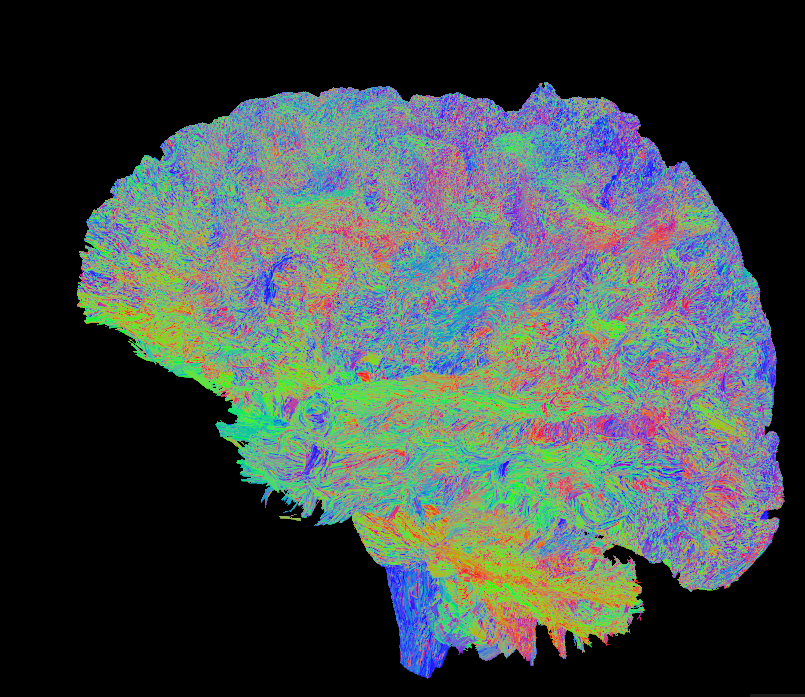
\includegraphics[height=0.9\textwidth,width=0.9\textwidth]{images/tractography.png}
         \caption{Tractography}
         \label{fig:1M_tract}
     \end{subfigure}
    \hfill
     \begin{subfigure}[b]{0.4\textwidth}
         \centering
         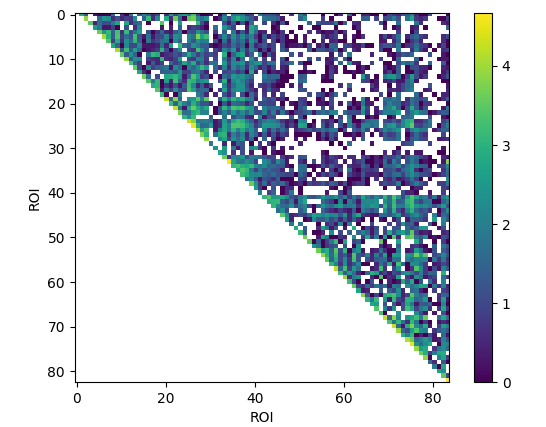
\includegraphics[height =0.9\textwidth,width=\textwidth]{images/connectome_1M.png}
         \caption{Connectome}
         \label{fig:connectivity_matrix}
        \end{subfigure}
    \vfill
        \begin{subfigure}[b]{0.6\textwidth}
         \centering
         \vspace{2em}
         %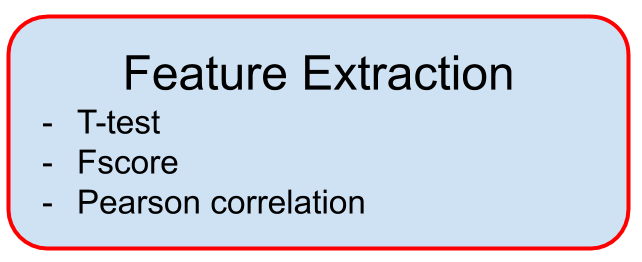
\includegraphics[height=0.3\textwidth,width=0.5\textwidth]{images/Features_1.png}
        \begin{tcolorbox}[box align= center,coltitle=black!75!black, colback=yellow!5!white,colframe=yellow!50!black,
  colbacktitle=yellow!80!black,title=\centering \large Feature Representation]
        \centering
        f-scores, t-test, Pearson correlation
        \end{tcolorbox}
        \caption{}
         \label{fig:feature extraction}
         \end{subfigure}
    \vfill
    \begin{subfigure}[b]{0.9\textwidth}
    \begin{subfigure}[b]{0.3\textwidth}
        \begin{tcolorbox}[coltitle=black!60!black ,colback=yellow!5!white,colframe=yellow!50!black,
  colbacktitle=yellow!75!black, fontupper=\color{black}, title=\centering \large Feature Selection]
        Select k\% features
        \end{tcolorbox}
         %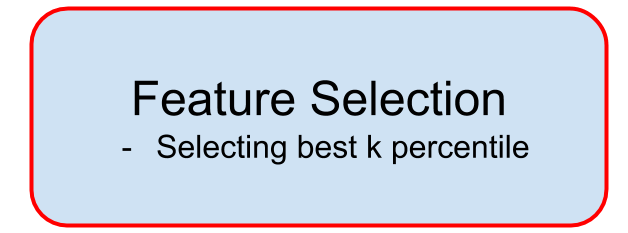
\includegraphics[height =0.8\textwidth,width=\textwidth]{images/Features_2.png}
         \vspace{1cm}
         \label{fig:feature selection}
         \end{subfigure}
    \hfill
    \begin{subfigure}[b]{0.4\textwidth}
         \centering
         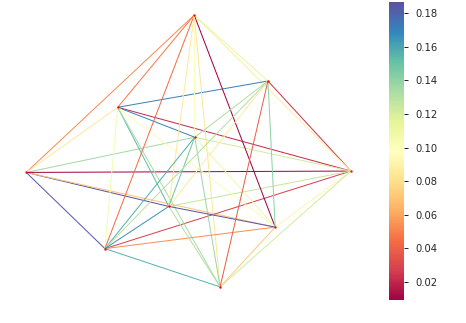
\includegraphics[height =0.8\textwidth,width=\textwidth]{images/mews.png}
         \label{fig:mewspip}
         \end{subfigure}
    \vspace{-2em}
     \caption{Feature selection using either baseline analysis or MEWIS solver.}
    \end{subfigure}
    \vfill
        \begin{subfigure}[b]{0.6\textwidth}
         \centering
         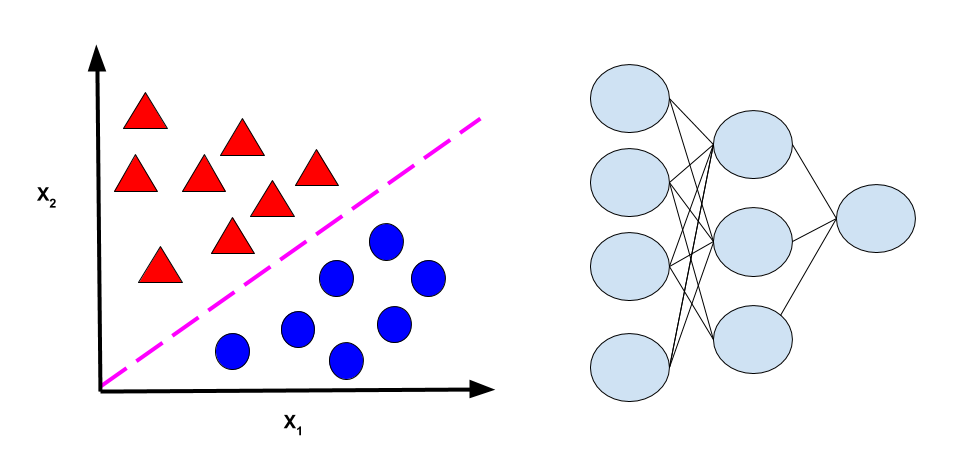
\includegraphics[height =0.4\textwidth,width=\textwidth]{images/classification.png}
         \caption{Classification}
         \label{fig:three sin x}
         \end{subfigure}
    \caption{Summary of the pipeline implemented in this thesis. (a) Whole brain, one million streamlines tractography computed for each subject. (b) Connectivity matrix encoding DWI information. In this case, the matrix represents the number of streamlines between any two regions of interest in the $log_{10}$ scale. (c) Different statistical measures used to represent the importance of the original features present in the dataset. (d) Ranking of edge importances using two different techniques. Baseline selects according to percentile distribution and MEWIS solver extracts a predictive subgraph. (e) Classification using \gls{SVM}s, \gls{RF2}s and \gls{MLP}s.}
    \label{fig:pipeline}
\end{figure}

A classification task was designed for the MRI data from the \gls{HCP}. The pipeline for designing this classification task consisted of four major steps. First a whole brain tractography was generated on the basis of \gls{DWI} scans for each subject. Then, three types of connectomes were created for each subject and represented in the form of connectivity matrices. This was followed by deployment of two different feature selection techniques for classification of subjects based on the connectivity matrices: namely `baseline' and \gls{MEWIS}. Finally, machine learning classifiers were used to test the effectiveness of these two feature selection techniques. The summary of the pipeline is presented in \autoref{fig:pipeline}.

The implementation of this pipeline was scripted in \textit{Python}. The preprocessing of the \gls{HCP} data to generate tractography was done with the help of \textit{MRtrix3} (\cite{tournier2019mrtrix3}). Data was prepared in a classification ready format using \textit{Pandas} (\cite{mckinney2011pandas}) dataframes. The Maximum Edge Weight k-Induced Subgraph problem was implemented in \text{Java} based on a modification from \cite{DBLP:journals/corr/LobodaAS16} (\href{https://github.com/ctlab/gmwcs-solver}{\textbf{\textit{github.com/ctlab/gmwcs-solver}}}). The final classification was based on machine learning implementation from \textit{scikit-learn} \citep{sklearn_2012}. 

\section{Data Acquisition}
\label{sec:acquisition}
Structural and \gls{dMRI} data for 203 subjects was acquired from the s900 release of the \gls{HCP} (\cite{hcp2015wu}). Out of the total, 101 subjects were females and 102 were males. 83 females and 58 males were aged 26-30 and remaining 34 males and 28 females were aged 22-25. The demographic information along with other markers of emotion and cognition were obtained from the unrestricted access data available on \href{https://db.humanconnectome.org/}{\textbf{\textit{https://db.humanconnectome.org/}}}.

\subsection{Imaging Data}
\begin{table}[h!t]
\begin{tcolorbox}
    \centering
    \begin{tabular}{!{\vrule width 2pt}c|c!{\vrule width 2pt}}
    \specialrule{0.2em}{0.01em}{0.01em}
         TR (ms) & 2400\\
    \hline
         TE (ms) & 2.14 \\
    \hline
         T1 (ms) & 1000 \\
    \hline
         Flip angle & 8 deg \\
    \hline
         FOV & 224 x 224 \\
    \hline
         Voxel Size & 0.77 mm isotropic \\
    \specialrule{0.2em}{0.01em}{0.01em}
    \end{tabular}
    \caption{Acquisition parameters for the structural image acquired from the \gls{HCP} s900 release. }
    \label{tab:structuralmri}
\end{tcolorbox}
\end{table}
\begin{table}[h!]
\begin{tcolorbox}
\centering
    \begin{tabular}{!{\vrule width 2pt}c|c!{\vrule width 2pt}}
        \specialrule{0.2em}{0.01em}{0.01em}
         Sequence &  Spin-echo EPI \\
          \hline
         slice thickness & 1.25 mm, 1.25 mm isotropic voxels\\
          \hline
         TR (ms) & 5520  \\
          \hline
         TE (ms) & 89.5 \\
          \hline
         Flip angle & 78 deg \\
          \hline
         Refocusing flip angle & 180 deg \\
          \hline
         FOV & 224 x 224 \\
          \hline
        Voxel Size & 0.77 mm isotropic \\
         \hline
        b-values & 100,2000 and 3000 $s/mm^2$\\
        \specialrule{0.2em}{0.01em}{0.01em}
    \end{tabular}
    \caption{Parameters for the acquisition of Diffusion MRI data acquired from the \gls{HCP}.}
    \label{tab:diffusionmripara}
\end{tcolorbox}
\end{table}
The structural and \gls{dMRI} files used for this project were obtained from the repositories containing images processed using version 3 of the preprocessing pipelines in the \gls{HCP} detailed in \cite{GLASSER2013105}. A Siemens 3T Skyra system was used used to scan all subjects (starting in August 2012, housed at Washington University, St. Louis). The details of the acquisition protocol are can be obtained from \cite{van2012human}.

In order to accomplish the goals of this project, there were two types of structural images acquired for each subject from the \gls{HCP} pipeline. The first type was an image consisting of a segmentation volume along with cortical surface parcellation based on the Desikan Killiany Atlas \citep{desikan2006automated}. The second type was the T1w scan in subject space. This anatomical images was aligned to the location at the interface of hemispheres: \gls{AC-PC}. This \gls{AC-PC} alignment is a rigid body rotation so that the image gets `centered' and can be termed as registration. The image was sampled at the same resolution as the diffusion data (1.25 mm isotropic, originally 0.77 mm isotropic). The parameters of the T1w images are presented in \autoref{tab:structuralmri}.

The important characteristics of the \gls{dMRI} images acquired is that they were obtained in very high resolution (1.25 mm isotropic) using a Stejskal-Tanner (monopolar) diffusion encoding scheme as mentioned in \autoref{sec:DWI}. The q-space was sampled by including 3 shells at the b-values presented in \autoref{tab:diffusionmripara} with each gradient table defined by a single b-value acquired once with right-to-left and another in the opposite phase encoding polarities. For each subject, four types of DWI files were acquired: preprocessed diffusion time series, the brain mask in diffusion space,  diffusion weighting for each volume and diffusion direction for each volume.


\subsection{Label Preparation}
\label{sec:label_preparation}
\iffalse
\begin{table}
\label{table:personality}
\begin{tabular}{|l|l|l|l|l|l|}
\hline
&Agreeableness&Openness&Conscientiousness&Neuroticism&Extraversion\\
\hline
count&203.0&203.0&203.0&203.0&203.0\\
\hline
mean&32.103&28.759&34.65&17.133&30.901\\
\hline
std&5.442&6.074&5.939&7.67&5.901\\
\hline
min&13.0&12.0&12.0&0.0&12.0\\
\hline
25\%&29.0&25.0&31.0&12.0&27.0\\
\hline
50\%&32.0&28.0&35.0&17.0&31.0\\
\hline
75\%&36.0&33.0&39.0&22.0&35.0\\
\hline
max&45.0&45.0&48.0&43.0&46.0\\
\hline
\end{tabular} (make a histogram maybe)
\caption{Summary of personality traits for all subjects.}
\end{table}
\fi 


\begin{table}[h!b]
\begin{tcolorbox}
\begin{tabularx}{\textwidth}{!{\vrule width 2pt}X|X|X|X|X|X !{\vrule width 2pt}} \specialrule{0.2em}{0.01em}{0.01em}
\textbf{}& \textbf{Agreeab-}& \textbf{Openness} &\textbf{Conscien-}& \textbf{Neurotic- }& \textbf{Extraver-}\\
                   &\textbf{leness  }&       &\textbf{tiousness } & \textbf{ism} & \textbf{sion }\\
 \specialrule{0.2em}{0.01em}{0.01em}
count&141.0&141.0&141.0&141.0&141.0\\
\hline
mean&32.482&28.326&35.262&16.965&30.766\\
\hline
std&5.144&6.021&5.615&8.046&5.918\\
\hline
min&13.0&12.0&21.0&0.0&18.0\\
\hline
25\%&30.0&25.0&31.0&12.0&27.0\\
\hline
50\%&33.0&28.0&36.0&17.0&31.0\\
\hline
75\%&36.0&32.0&39.0&21.0&34.0\\
\hline
max&44.0&43.0&47.0&43.0&46.0\\
 \specialrule{0.2em}{0.01em}{0.01em}
\end{tabularx}
\caption{Summary of personality traits for training data subjects.}
\label{table:personality}
\end{tcolorbox}
\end{table}
The generalized pipeline implemented in this work could be used with different types of variables. Results for the big5 personality traits and gender are presented in the results section. Each of these labels were dealt with in a different manner.

The big5 personality traits are continuous. The statistical description of the personality traits for the training subjects is represented in \autoref{table:personality}. Personality traits are based on the five factor model of personality (\cite{costa1992five}). The five different personality traits are agreeableness, conscientiousness, neuroticism, extraversion and openness. They are often used in psychology and psychiatry to characterize behavior.

The architecture of the pipeline of this work required the conversion of the continuous label prediction to a classification task. The conversion steps were as follows:
\begin{enumerate}
\item Record the median of the personality trait the training subjects.
\item Divide the personality labels into 5 quartiles.
 \item Remove the data of the subjects whose personality traits fall into the middle quartiles.
 \item Binarize the variables such that the first two quartiles belong to the lower class and the last two quartiles correspond to the higher class.
\end{enumerate}

The gender variables were categorical. For the classification task, male attribute was mapped to zero and females to one.

\section{Creating the Connectome}
\label{sec:creating_connectome}

A connectome for each subject was generated on the basis of tractography. The nodes of the connectome were determined using a parcellation mask as elaborated in \autoref{sec:connectomics}. This workflow was implemented on the basis of the tutorial titled ``\textit{ISMRM tutorial - Structural connectome for \gls{HCP}}''
\iffalse(\href{https://mrtrix.readthedocs.io/en/latest/quantitative_structural_connectivity/ismrm_hcp_tutorial.html}{\textbf{\textit{https://mrtrix.readthedocs.io/\\en/latest/quantitative\_structural\_connectivity/ismrm\_hcp\_tutorial.html}}})\fi. The preparation of the structural connectivity matrices has been visualized in \cref{fig:connectome_pipeline}. The subsquent subsections will explain the two parallel procedures for structural and diffusion images respectively which are combined to generate the connectome file. 
\begin{figure}
    \centering
    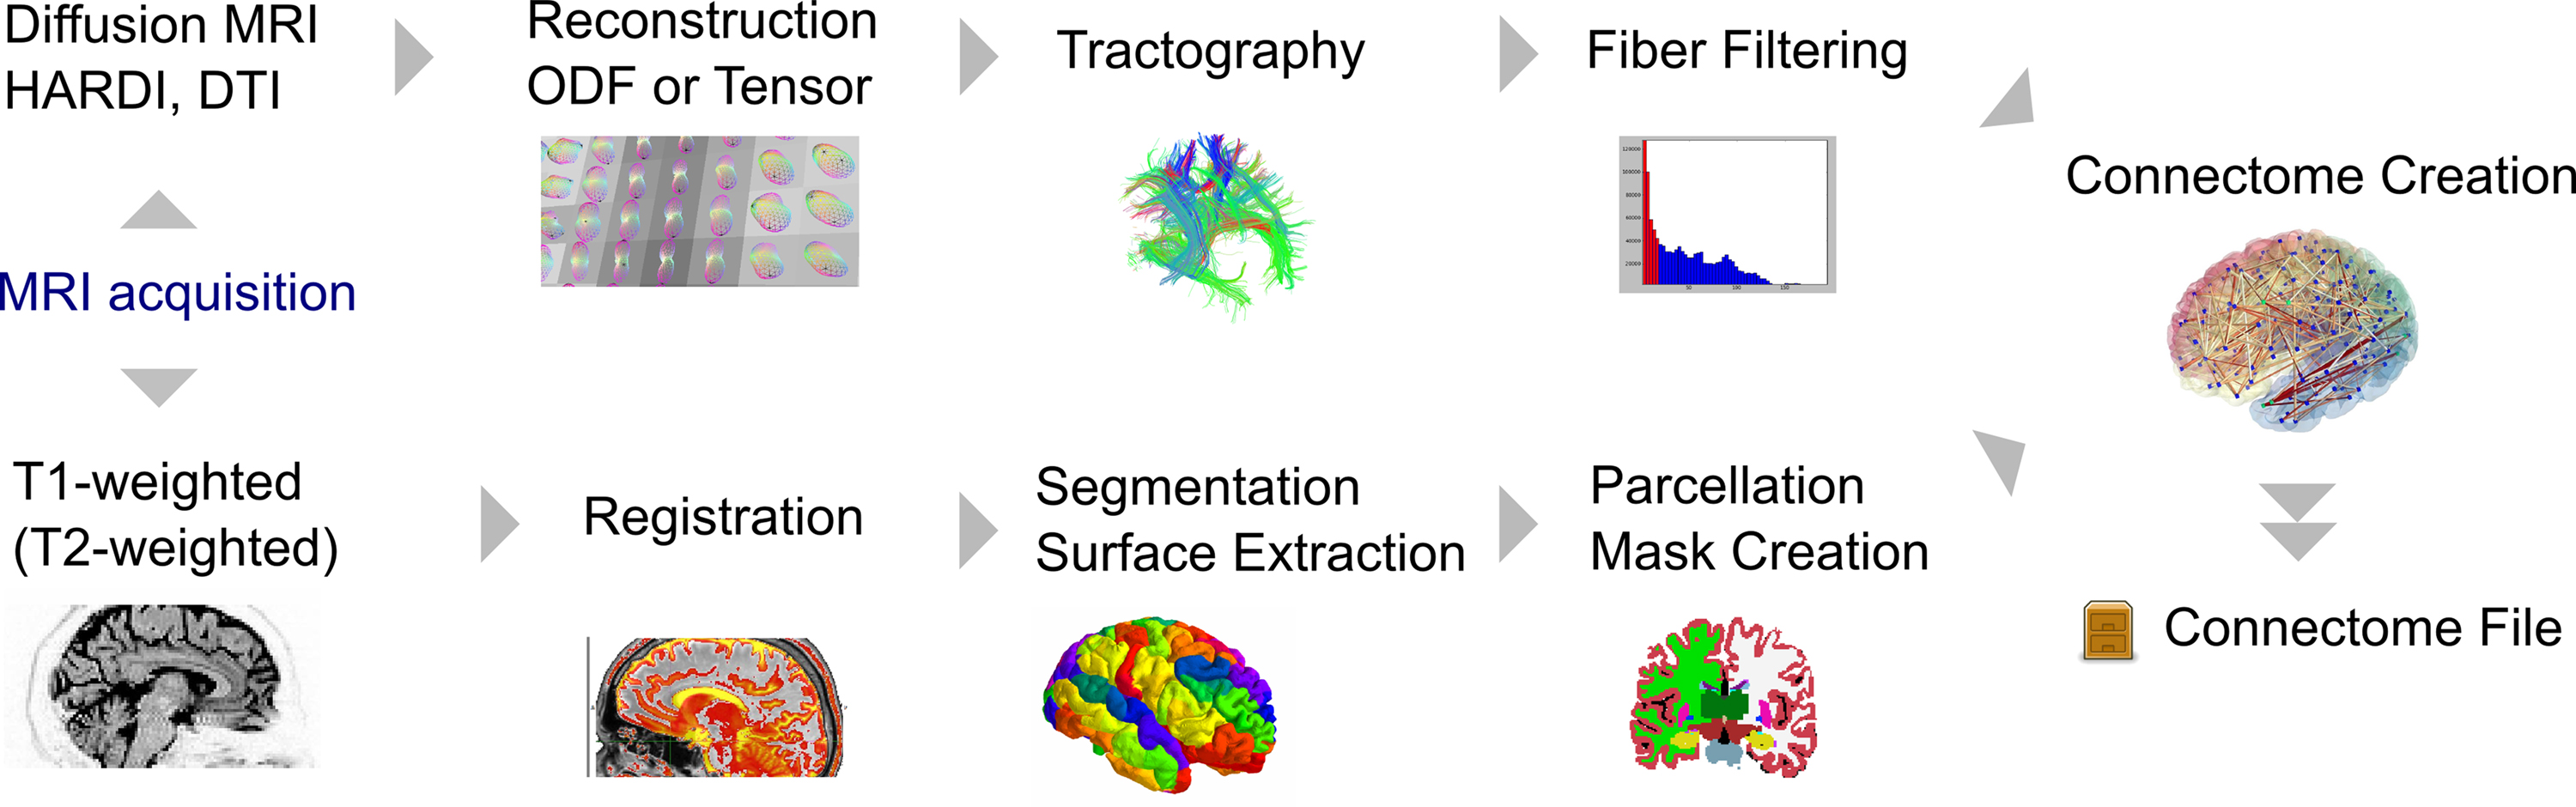
\includegraphics[width=\textwidth]{images/connectome_creation_workflow.png}
    \caption{Pipeline for creating the connectome for each subject. Two parallel workflows following data acquisition have been illustrated in this figure. The first procedure aims to extract a parcellation mask from the structural images of each subject in their native space. The second `parallel' procedure generates anatomically correspondent tractograms from diffusion images. A connectome file is generated after combining the information from filtered tractograms and parcellation mask. The connectome file contains properties of the fibers that connect \gls{ROI}s determined by the parcellation mask. Image from \cite{gerhard2011connectome}.}
    \label{fig:connectome_pipeline}
\end{figure}
\subsection{Structural Image Processing}
\label{subsec:struct_diff}
The end goal of the structural image processing was to generate a parcellation mask indicating gray matter ROIs. The steps of the structural image processing in \cref{fig:connectome_pipeline} were readily accomplished by the \gls{HCP} preprocessing pipeline \citep{GLASSER2013105}.

The registered T1w images along with the segmentation surfaces and parcellation msks were available within the \gls{HCP} data (\autoref{sec:acquisition}). The T1w images were registered according to the rigid transformation for making the image centered along anterior-posterior commisure. The segmentation surfaces were labelled according to FreeSurfer's default subcortical segmentation consisting of 9 \gls{ROI}s
\iffalse namely: caudate, pallidum, hippocampus, lateral ventricle, putamen, amygdala, thalamus, nucleus acumbens and the cerebellum\fi. The parcellation was based on FreeSurfer's automatic cortical parcellation according to the Desikan-Killiany atlas that delineates 35 \gls{ROI}s. The combined parcellation and segmentation image was available from the \gls{HCP} data was used to generate a volume delineating locations of the nodes of the connectome or \gls{ROI}s. 

FreeSurfer's default lookup table for the labels of \gls{ROI}s was not linear. The nodes of the original `combined' image were then mapped to the default lookup table in \textit{MRtrix3}. This made the numbering of the ROIs (also the nodes of the connectome) start from 1. Furthermore, FreeSufer's estimates of sub-cortical grey matter structures were replaced with the estimates from FSL's FIRST tool.
The nodes of the generated connectome were labelled according to the default lookup table in \textit{MRtrix3}. There were 8 subcortical gray matter regions (the accumbens area was incorporated into thalamus label) and 34 cortical gray matter ROIs (see Appendix). 

It is important to note that along with the diffusion data, the structural data was also used for probabilistic whole-brain tractography \citep{parker2003framework}. Hence, in addition to generation of a combined parcellation mask, a \gls{5TT} segmented image was also generated. This was done on the basis of sampling the T1w structural volume in the subject's native space at the same resolution as the diffusion data (1.25 mm isotropic). The 5TT image delineated the segmentation of brain regions into five tissue types; namely gray matter, subcortical gray matter, \gls{WM}, \gls{CSF} and pathological tissue. The segmentation is based on FSL segmentation tools FIRST and FAST. This information about the location of different tissue types makes the tracking based on DWI images suitable for \gls{ACT} \citep{anattractsmith}.
\iffalse
The diffusion image was first converted to a non-compressed format. The information about the diffusion gradient encoding was represented in the header of the file, the volume data was made continuous voxel-wise and the data points were converted to a floating point format. 
After this, the mean b=0 image was generated for visualization. The b=0 image serves as a sort of baseline for anatomical reference.

The multi-shell, multi-tissue response function was determined  in order to form Multi-Shell, Multi-tissue spherical deconvolution. 

Atleast three unique b-values are required to estimate three tissue comparments. These 
The deconvolution leads to the formation of a 4 dimensional image in which each 3D volume (as viewed in \comment{part of pipeline figure in preprocessing} is RGB encoded where the cerebrospinal fluid (CSF) is seen in red, the gray matter in green and the white matter in blue. 
\fi

\subsection{Diffusion Image Processing}
\label{sec:Diffusionimgprepro}
\iffalse
The second ’parallel’ procedure of generating filtered tractograms was implementedin the pipeline of this work.
\fi
The first step of processing the diffusion images was to determine the local fiber directions in order to prepare for probabilistic tractography. In order to accomplish this task the response functions of the \gls{WM}, \gls{GM} and \gls{CSF} were extracted from the five-tissue type (5TT) image. From the Contrained Spherical Deconvolution (CSD) of the response function and the DWI image the \gls{fODF}s were reconstructed based on  the algorithm in \cite{jeurissen2014multi}. 

\iffalse
\gls{fODF}s were reconstructed using \gls{MSMT-CSD} based on the algorithm in \cite{jeurissen2014multi}. As mentioned in  \autoref{sec:highermodels} the \gls{CSD} of response functions can determine the fODF distribution. of the separate response functions from WM, GM and CSF was done in order to obtain the DWI signals of the three tissue types from the 5TT image.
\fi

The probabilistic whole-brain tractography of five-million fiber tracts was generated using the white matter fiber orientation distributions. Tractography was performed in the subject space since a structural image in this space is the best approximation of the subject's physical brain. The streamlines were computed on the basis of the algorithm iFOD2 \citep{tournier2010improved}. This algorithm uses the \gls{fODF} image and determines candidate streamline paths (arcs), which have greater \gls{fODF} amplitudes along the paths. By sampling the underlying \gls{fODF} amplitudes along these arcs it makes the streamlines likely to follow most probable paths.

Anatomical constraints on the tractography were provided using the \gls{5TT} image. There were other series of constraints imposed in order to make the  tractography more informed. The seed points were dynamically determined using the \gls{SIFT} model \citep{smith2013sift} of the white matter fODFs. The cutoff value of $0.06$ was set for the probability amplitude for terminating tracks. The maximum length of streamlines was set at 250 mm i.e. 200 times the voxel size in our case where the voxel size is 1.25mm. The tracking along a streamline was truncated if the fiber terminates at poor structural location and  retracking was performed. The streamlines were cropped whenever they cross the grey matter-white matter interface. 

The tractography was downsampled from five million fibers to one million fibers to preserve the most biologically relevant fibers using the SIFT algorithm \citep{smith2013sift}. This provided more meaningful estimates of the structural connection density and also reduced the memory requirements. 

\subsection{Connectome Representation}
\label{subsec:connectomegeneration}
The connectome can be represented in the form of a graph as mentioned in \autoref{sec:connectomics}. After obtaining the tractography and a parcellation image representing the subject specific node locations of the connectome, the connectome matrix was obtained in a \textit{.csv} format. It was generated from the whole brain tractography of one million tracts using 84 relevant grey matter parcellations (see   Appendix).

The 84 nodes represent a 8 subcortical gray matter ROIs and 34 cortical gray matter ROIs with each ROI contributing to two nodes (one in the left hemisphere and another in the right hemisphere). Using different parameter settings three types of features were extracted. The mean \gls{FA} (Eq. \ref{eq:meanFA}), the average length and number of streamlines between any two regions. The visualization can be seen in the \autoref{fig:connectivity_matrix}. The connectome is represented as an upper triangular matrix ($84 \times 84$, corresponding to $3570$ features) considering that the connections between two ROIs are symmetric.

\iffalse
In the  it can be seen that there is a need to decipher the streamlines which are terminating in the specified regions of interest
\fi
\section{Feature Representation}
\begin{figure}
    \centering
    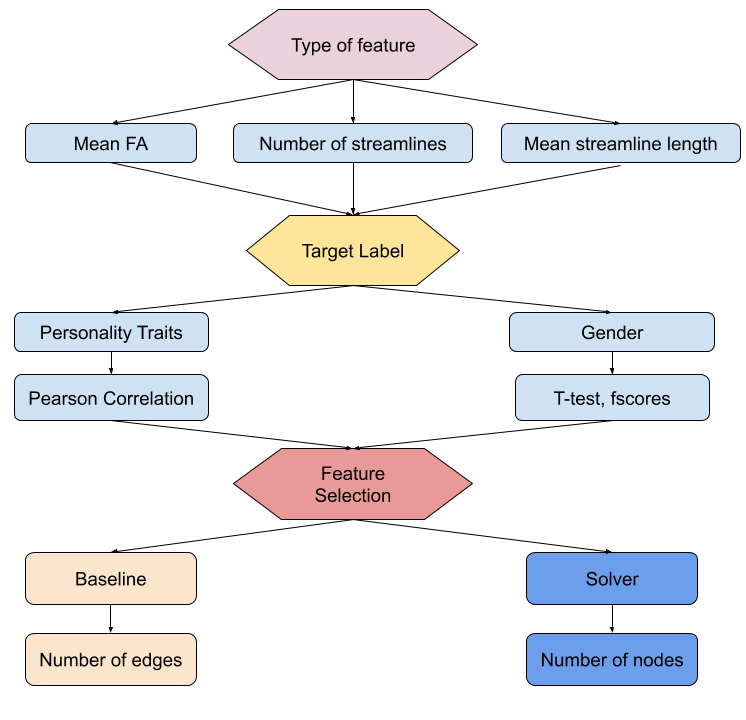
\includegraphics[width=\textwidth]{images/Graph_clf_possibilites.png}
    \caption{Considerations for classification task. Each path along this graph represents a different possibility for a classifier to be trained on. The parameters for training the classifier are: the type of feature, the target label and the feature selection technique.}
    \label{tab:classify_combo}
    %\label{fig:my_label}
\end{figure}
\iffalse
\begin{table}[ht]
\begin{tcolorbox}
\centering
    \begin{tabular}{|p{0.15\textwidth}|p{0.3\textwidth}|p{0.3\textwidth}|p{0.1\textwidth}|}
        \specialrule{.2em}{.05em}{.05em}
        Target labels & \multicolumn{3}{c}{Personality metrics | Gender}\\
        \specialrule{.2em}{.05em}{.05em}
         Type of feature & Mean \gls{FA} & Number of streamlines & Mean streamline length \\
         \specialrule{.1em}{.05em}{.05em}
        Edge representations & Pearson correlation coefficient &  t-test & f-scores\\
        \specialrule{.1em}{.05em}{.05em}
        Feature &  \multicolumn{3}{c}{Solver | Baseline}\\
        Selection & Number of nodes & Percentage of features\\
        & [4...30]  & {2,5,10,50,100} \\
        \specialrule{.2em}{.05em}{.05em}
     \end{tabular}     
    \caption{Considerations for classification task.}
    \label{tab:classify_combo}
\end{tcolorbox}
\end{table}
\fi

Once the connectivity matrices for all the 201 subjects were computed and encoded in the format of a .csv file, a \textit{pandas} \textit{dataframe} was prepared to serve as input to the classifier. Each row represented the data for an individual subject. Each column represented the connection between any two brain regions i.e. features in one cell of the connectivity matrix. Three different types of features obtained using the connectome files according to \autoref{subsec:connectomegeneration}. The design of the classification task was based on different attributes presented in \autoref{tab:classify_combo}. A classifier was trained on one set of configurations for two different feature selection techniques. The details will be discussed in the subsequent subsections.

Self-loops were omitted from the analysis pipeline due to incompatibility with the solver based implementation and non-significant changes to classification accuracy based on the omission. Furthermore, using the calculation of statistical coefficients on the raw data the importance of each feature was determined. 

The training set consisted of 141 subjects consisting of 83 females and 58 males aged 26-30. While the independent test set consisted of 34 male and 28 females aged 22-25. The data was standardized using \textit{sklearn} by removing the mean and scaling to unit variance since the different types of features were in separate scales of magnitude.

\subsection{Statistical Coefficients}
\label{subsub:statcoef}
The raw features were not representative of any information on a group level. To gain information about feature importance statistical coefficients were used. From the raw matrices, each column was be represented as a statistic and hence `group averaged' edge of the connectivity graph. 

Statistical coefficients are effective feature filter methods for the classification from Neuroimaging data. Filter methods were used since they can be retraced to the original features. Mainly, three coefficients were used. The first two were the t-test and the f-scores,which describe the discriminative power of a particular feature. The Pearson correlation coefficient was used in the case of continuous variables to capture the linear relationships between the features and the target values. In order to rank the features an absolute value of the Pearson coefficient was used to highlight its importance.The f-score used in the analysis is used to measure how well the particular feature distinguishes between the two classes labelled as 1 and 2. It was calculated according to \cref{eq:fscores}. 

The t-test was processed as differently depending on the size of the classes. In the case of personality traits, size of both the classes was the same since the personality traits were binned according to the median (\autoref{sec:label_preparation}). An independent samples t-test according to \cref{eqn:tstat ind} was carried out for feature selection. For gender classification the sample size for both classes was different, the training set consisted of 83 females and 58 males. In this case an Welsch's t-test assuming similar variance was carried out (Eq. \ref{eqn:tstat welsch}). The p-value of the t-test was used to determine it's statistical significance by converting it into the $log_{10}$ scale. Each p-value $p_x$ was represented by $ f(p_{x}) = (-1) \times \log_{10} p_x$ so that a higher numerical value represents a higher statistical significance. 
\subsection{Exclusion of Self Loops}
\label{sec:exclusion}
Self loops can be termed as the connections from the brain regions to themselves. They were excluded from the analysis before feeding data to the classifier. These loops were incompatible with the \gls{MEWIS} implementations and hence they were removed from baseline analysis performance comparison between the two methods. Further, this exclusion will be justified by the performance of the classifiers with and without the inclusion of self-connections between the ROIs in \autoref{res:selfloops}. 

Their exclusion was an important consideration for the \gls{MEWIS} solver based implementation. Degenerate edges are not part of a simple graph, their inclusion was incompatible with the implementation from \cite{DBLP:journals/corr/LobodaAS16}. After removing such connections the \gls{MEWIS} implementation was able to solve the \gls{MIP} formulation and produce subgraphs.

The results in \autoref{res:selfloops} help evaluate the importance of self loops was ascertained by seeing their effects on classification metrics. This is done on the basis of a paired samples t-test. The first sample is taken as the classification performance on the  data including the self loop features. Alternatively, the second sample is the classification performance obtained by excluding self loops. In general, the null hypothesis of a paired sample t-test remains that the differences between the observations from two samples is zero. Two slightly different experiments were carried out for classification of personality traits and gender. The formulas for calculation however remain the same. The t-statistic is calculated by:

\begin{align}
    \label{eq:pairedtest}
    t = \frac{\Tilde{X_{D}} - \mu_0}{\frac{s_{D}}{\sqrt{n}}} \\
    \Tilde{X_D} = \sum_{i=1}^{N} \frac{a_{i} - b_{i}}{n}
\end{align}where $s_D$ is the standard deviation of the differences between the metrics of the experiments with the self loops $a$ and without the self loops $b$. Arrays $a$ and $b$ have the same length $n$. There was one entry in the array for each possibility in a combination of choice for different attributes:
\begin{itemize}
    \item Classification label
    \item Percentage of features in the set: $[2,5,10,50,100]$
    \item Three different classifiers: MLP, support vector machines, and random forest classifier 
    \item Edge type (representatives of raw features, \autoref{subsub:statcoef}): depending on classification label
\end{itemize}

The null hypothesis for classification of personality traits was that the average of a particular classification metric on the basis of one feature (such as mean \gls{FA}, mean streamline length and number of streamlines) is the same. Including data for all five personality traits and one type of edge for arrays $a$ and $b$ had a size  $n=75$ i.e. $5\times 5 \times 3 \times 1$. 

In a similar fashion, the null hypothesis for the gender based classification was the same. However, instead of five personality traits there was one label used i.e. gender and two edge type (t-test and f-scores). This resulted in $n=30$ i.e. $1 \times 5 \times 3 \times 2$.

The null hypothesis could not be rejected because for the test data, the p-values of these t-tests were high. This indicates that the difference between the classification on the data with and without the self loops is not statistically significant. Self loops could hence be safely eliminated and the results of these experiment are presented in \autoref{res:selfloops}. After the elimination of the self loops that correspond to the diagonal of $84 \times 84$ connectivity matrix, there was a total of $n = 3486$ features for each subject.

\section{Feature Selection} 
The motivation to perform feature selection from considerations of time complexity and removal of redundant features. There were two types of feature selection techniques used before classification. The first one was a classical feature selection technique based on statistical coefficients and is termed as the `baseline'. The second technique was based on extracting a subgraph after converting the original edge weights to statistical coefficients and is termed as the `solver' method based on the \gls{MEWIS}. 

The \gls{MEWIS} technique produces more interpretable results as compared to filter methods due to incorporation of graph topology. It is proposed due to the fact that analyzing the inter-subject differences at the subnetwork level is easier than analyzing dense subgraph of whole brain connectivity. 

\subsection{Baseline Analysis}
\label{subsec:Baseline_ana}
% Question: which one do we report? Solver was working only with the Pearson correlation coefficient.

Baseline experiments were solely based on the filter methods mentioned in \autoref{sec:feature_selection}. In this technique, there is no information about graph topology or the biological correspondence of the features. Feature importance is determined purely on numerical values.

For each of the structural connections, the statistical coefficient was calculated based on the data and target variables from the training set. The metrics mentioned in \autoref{subsub:statcoef} were then used to rank the features. This ranking was based on first taking the absolute value of the coefficients and then dividing the coefficients for all features into a percentile distribution. This gave a ranking from which the top percentiles were selected according to a parameter $k$. Initially, $k \in \{2,5,10,50,100\}$ were chosen to cover the  overall trend of classifier performance as a function number of features. Later in the course of multiple experiments, this parameter $k$ could be adjusted according to requirements for comparison to the number of features extracted by the \gls{MEWIS} solver.

\iffalse
The Pearson correlation coefficient was computed between the values of the feature for the training subjects and their corresponding personality trait values. It was a trial to capture the linear relationship between a parameter (such as mean \gls{FA}) representing a brain connection and the outcome label (i.e. personality trait).

The f-score based selection was done by computing the f-score between the feature values for the training set and thresholded values of the target variables according to the median of the training data labels. 

The f-scores served as feature filtering step for the baseline experiments as they were used by dividing the f-score distribution into percentiles and then choosing the percentage of features we want in the specified top percentile. However, for the solver based experiments the f-scores for each feature was (numerically) low which made the MIP problem hard to run computationally. Even multiplying the f-scores with an order of $10^3$ was not useful since the standard deviation of the f-scores was not too high (insert the standard deviation). 

This feature selection was in fact quite useful for the feature selection in the baseline experiments. The p-value of the t-test could be divided into percentile distributions and the top percentiles could be chosen accordingly. However, for the solver based experiments this selection did not work well due to computational effort. 

The Pearson correlation coefficient in fact did work because it considers the linear nature of the personality trait coefficients. This type of feature selection is well reported in literature for Neuroimaging data considering continuous variables. It performed well for the baseline experiments as well as the solver based feature selection. For both the cases the absolute value of the Pearson correlation coefficient was taken because only the correlation was important, whether it is positive or negative correlation was not a matter of concern for the analysis.

The f-score and the t-test were based on the binarization of the target variables according to the median values of the feature from the training set, this might lead to information loss and hence their lower numerical values. 
\fi

\subsection{Maximum Edge Weight k-Induced Subgraph}
\label{method:MEWS}

The Maximum Edge Weight k-Induced Subgraph (MEWIS) problem is defined as the extraction of a subgraph induced by preserving $k$ nodes with a maximum total edge weight. The \gls{MEWIS} was taken as special case of the \gls{GMWCS} (\autoref{sec:MEWS}) for selecting graph based features in this pipeline. The implementation for the \gls{MEWIS} in this project was based on a modification of the Java application from \cite{DBLP:journals/corr/LobodaAS16} which made use of the IBM ILOG CPLEX Studio version 12.10 Java \gls{API}.The general explanation of the \gls{MEWIS} is as follows:

Consider an undirected graph $G=(V,E)$, then the aim is to find an induced subgraph $\tilde{G} (\Tilde{V}, \Tilde{E})$ with the set of vertices $\Tilde{V} \subset \Tilde{V}$ such that $\|\Tilde{V}\| = k$, $\tilde{G}$ is connected and has a maximized sum of edge weights \\ $\sum_{v \in \tilde{V}} w_e \longrightarrow max$. 

The generalized Maximum Weight Connected Subgraph (MCWS) was converted into the \gls{MEWIS} problem for a constant number of nodes. This was done by applying a constant negative weighting to all the nodes so that the subgraph which maximizes the \gls{MEWIS} condition can be found. Based on \cref{eq:sumfun} the \gls{MEWIS} condition was modelled as:
\begin{equation}
    \label{eq:sumews}
    \Phi (\Tilde{G}) = j \times m + \sum_{e \in \Tilde{E}} w_e \longrightarrow max \\
\end{equation}
where each node has a constant weight $j$ and the number of nodes corresponds to $m$. Such a technique was used for feature selection from structural brain connectivity as there is no predefined ranking for different regions of interest. The connections between two regions are important for the characteristics of the brain network. Detecting such a subnetwork in the brain can help analyze which set of nodes is responsible for differences between groups with regards to a particular target variable. 

All nodes in the input graph, $G(V,E)$, were given a constant negative weighting of $\{-0.01\}$ and all the edges obtained were positive since the absolute values of the coefficients in \autoref{subsub:statcoef} were taken. The small negative penalty was given to ensure a negative penalty on the inclusion of an extra node. Since all the edge weights were positive, the negative weights of the nodes ensured that the overall positive effect of the edge weights overcame the cost of keeping an extra node. This ensured the conservation of a specified number of nodes alongside compatibility for \gls{MEWIS}  (Eq. \ref{eq:sumews}). 

In the modification, giving the nodes a constant weight of zero results in all nodes getting preserved. This happened since there were no negative edges so none of the edges get eliminated. In this case the sum of all original edge weights remains the highest according to \cref{eq:sumews}. This effect was observed since the preprocessing step of the implementation in \cite{DBLP:journals/corr/LobodaAS16} was disabled and all nodes in the input graph remained well connected. Similarly, assigning any type of positive node weight is incompatible for the implementation in \autoref{method:MEWS} since no nodes and edges would get eliminated. 

The feature selection was carried out by making an input graph and a corresponding output graph. For each type of feature (mean FA, mean streamline length or number of streamlines), a graph was created specific to the target label of interest. The nodes in this graph correspond to ROIs mentioned in the appendix. The edges were the connections between the ROIs weighted by the statistical coefficients calculated for the training data with respect to the target variables. Such a graph was termed as the `input graph'. 

Sparsity to the input graph was introduced using two constraints. The absolute value of the edge weights (raw features represented by statistical coefficients, \autoref{subsub:statcoef}) shall not be zero. Simultaneously, features are conserved if and only if the tractography of each subject contains at least one streamline between the two nodes. 

For creating the output graph, parts of the pipeline used in \cite{DBLP:journals/corr/LobodaAS16} were modified. Constraints mentioned in \autoref{sec:MEWS} were extended and the additional constraint was to preserve a specified number of nodes using the constraint:
\begin{align}
    \label{eq:sum_constraints}
    \sum_{v=1}^{V} y_v = m        &&  \forall v \in V
\end{align}
where m is a controllable parameter specifying the number of nodes needed to be preserved in the output graph and $y_v$ is the binary variable mentioned in \autoref{eq:y_v}. The preprocessing module of the MCWS Java solver was disabled due to it's incompatibility with the required constraint (Eq. \ref{eq:sum_constraints}). This makes the subgraph produce an induced subgraph. 

An object oriented approach was taken to implement a class derived from the \textit{networkx} \citep{hagberg2008exploring} for the different input graphs and their corresponding output graphs. At any time, the graphs created for a specific use case could be read from text files and their properties could be explored.

In order compare the features selected with this technique to the baseline experiments, it was important to infer the number of edges being preserved based on a specific input configuration. The output number of edges was then analyzed as function of the number of nodes. The results are presented in \cref{fig:fun_num_edges}.

\section{Supervised Classification}

A Randomized Search 5-fold cross validation with implementation from \textit{scikit learn} was carried out for different algorithms in different cases based on the type of feature, the feature selection technique, target variables along with target labels are presented in \autoref{tab:classify_combo}. The cross validation was refitted using balanced accuracy on the test set. After the randomized search was finished, the best estimator was taken and fit to the training set. This classifier was then used to make predictions on an independent test set with difference in age range.

The training set consisted of 141 subjects, 83 females and 58 males aged 26-30. The independent test set consisted of 62 subjects, 34 males and 28 females aged 22-25. The different age ranges for the training and the test set were chosen in since the \gls{HCP} data contains scans of twins, but this information was available only from the restricted access of the data. Grouping the test and training set according to age ensured that both the twins remain in either the training set or the test set. If it was not done this way then the classification performance would become higher only due to similarity in features of one twin to another.

One model was trained each time there was a different configuration of settings presented in \autoref{tab:classify_combo}. Classification performance was assessed using the metrics \gls{AUC}, f1-score, accuracy and balanced accuracy.
\iffalse
The formulas of these metrics are based on the confusion matrix. An example confusion matrix for a binary classifier is:\\
\begin{equation}
\begin{bmatrix}
\begin{array}{c|c|c}
\hline
    & Predicted: No & Predicted: Yes \\
\hline
Actual: No & \textrm{\gls{TN}} & \textrm{\gls{FP}}\\
\hline
Actual: Yes & \textrm{\gls{FN}} & \textrm{\gls{TP}} \\
\hline
\end{array}
\end{bmatrix}
\end{equation}

\begin{align}
    \textrm{accuracy} &= \frac{TP + TN}{TP + TN} \\
    \textrm{Balanced accuracy} &= \frac{\frac{TP}{TP + FN} + \frac{TN}{TN + FP}}{2} \\
    \textrm{f1-score} &= \frac{TP}{TP + \frac{TP + FN}{2}}
\end{align}
\fi


\iffalse
\section{Visualization}
Since the graphs included in the analysis for each subject were dense. It was important to design effective visualization techniques for intuitively interpreting the features selected by the baseline and solver based method. 

\subsection{Chord Diagram}
A chord diagram is an effective way of visualizing the flow between different nodes. The connectome containing the feature of the number of streamlines that connect any two ROIs was represented a chord diagram created with the help of package \textit{holoviews} \citep{stevens2015holoviews}. Each ROI was represented as an entity or a fragment in the outer circle. The arcs drawn between the different node represent the connections and their thickness is proportional to the value of the number of streamlines in our case. In \cref{fig:connectome_num_streamlines} the average number of streamlines (for all subjects) between any two regions are visualized. There are multiple arcs connecting the two regions and these arcs get bundled and result in a thicker arc.

\subsection{Circular Diagram}
This visualization was specifically programmed illustrate different properties of the \gls{MEWIS} solver based technique. At first the features selected by the solver were traced back to the original \textit{dataframe} mentioned in 
visualization is \autoref{fig:gender_num_strls_10}.

\fi
\end{document}

